\chapter{Identifying Types of Load from Standing Wave Pattern\index{standing wave pattern}}\label{lec:lec9}

In the previous chapter, we discussed how to solve some simple common transmission line problems using both impedances and admittances and then we discussed the constant VSWR circle. In this chapter, we will discuss how to identify the types of load from standing wave patterns. Standing wave pattern has two important characteristics which are:
\begin{enumerate}[(i)]
\item The location of maximum and minimum (current/voltage)
\item The VSWR circle.
\end{enumerate}
So \emph{how can we quickly identify the type of load\footnote{The type of load is not the exact value of the load} without calculating the VSWR?}

Recall that:
\begin{align}
VSWR = \frac{|V|_\max}{|V|_\min}
\label{eqn:vswr09}
\end{align}
From the equation~\eqref{eqn:vswr09}, the smaller the value of $|V|_\min$, the larger the value of ${VSWR}$, that is, as $|V|_\min$ tends to zero, ${VSWR}$ tends to infinity. When $|V|_\max{\approx}|V|_\min$, then $VSWR = 1$.

First, let us observe the variation of the impedance on the tranmission line with the Smith Chart then we will revisit our early question. Figures~\ref{fig:group91} and~\ref{fig:group92} are simplified Smith Charts showing the VSWR circle for inductive and capacitive load at the top and bottom areas respectively.
\begin{figure}[h]
\centering
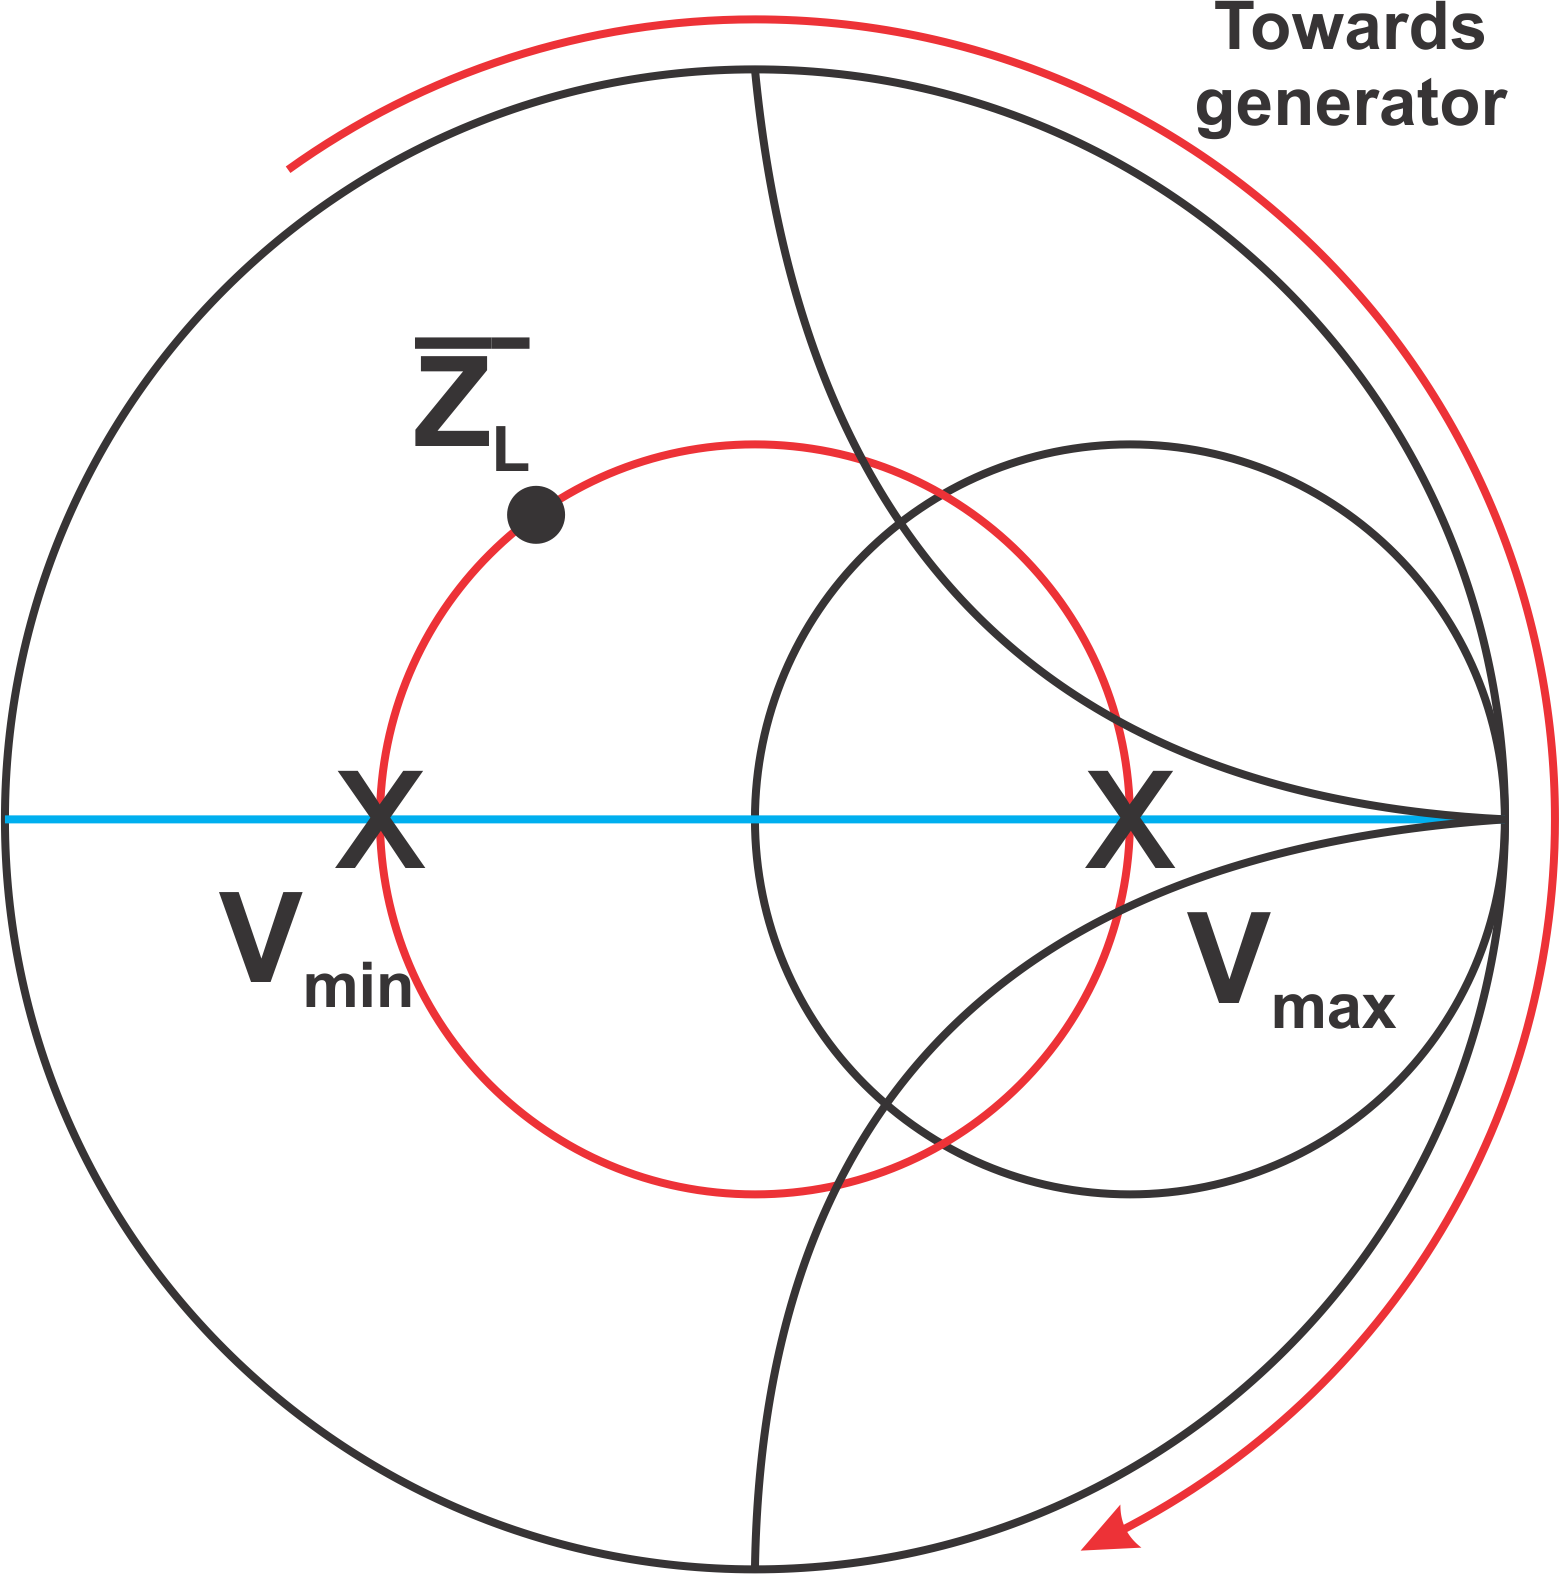
\includegraphics[scale=0.4]{./graphics/Group91}
\caption{A Smith Chart representation of inductive load}
\label{fig:group91}
\end{figure}
\begin{figure}[h]
\centering
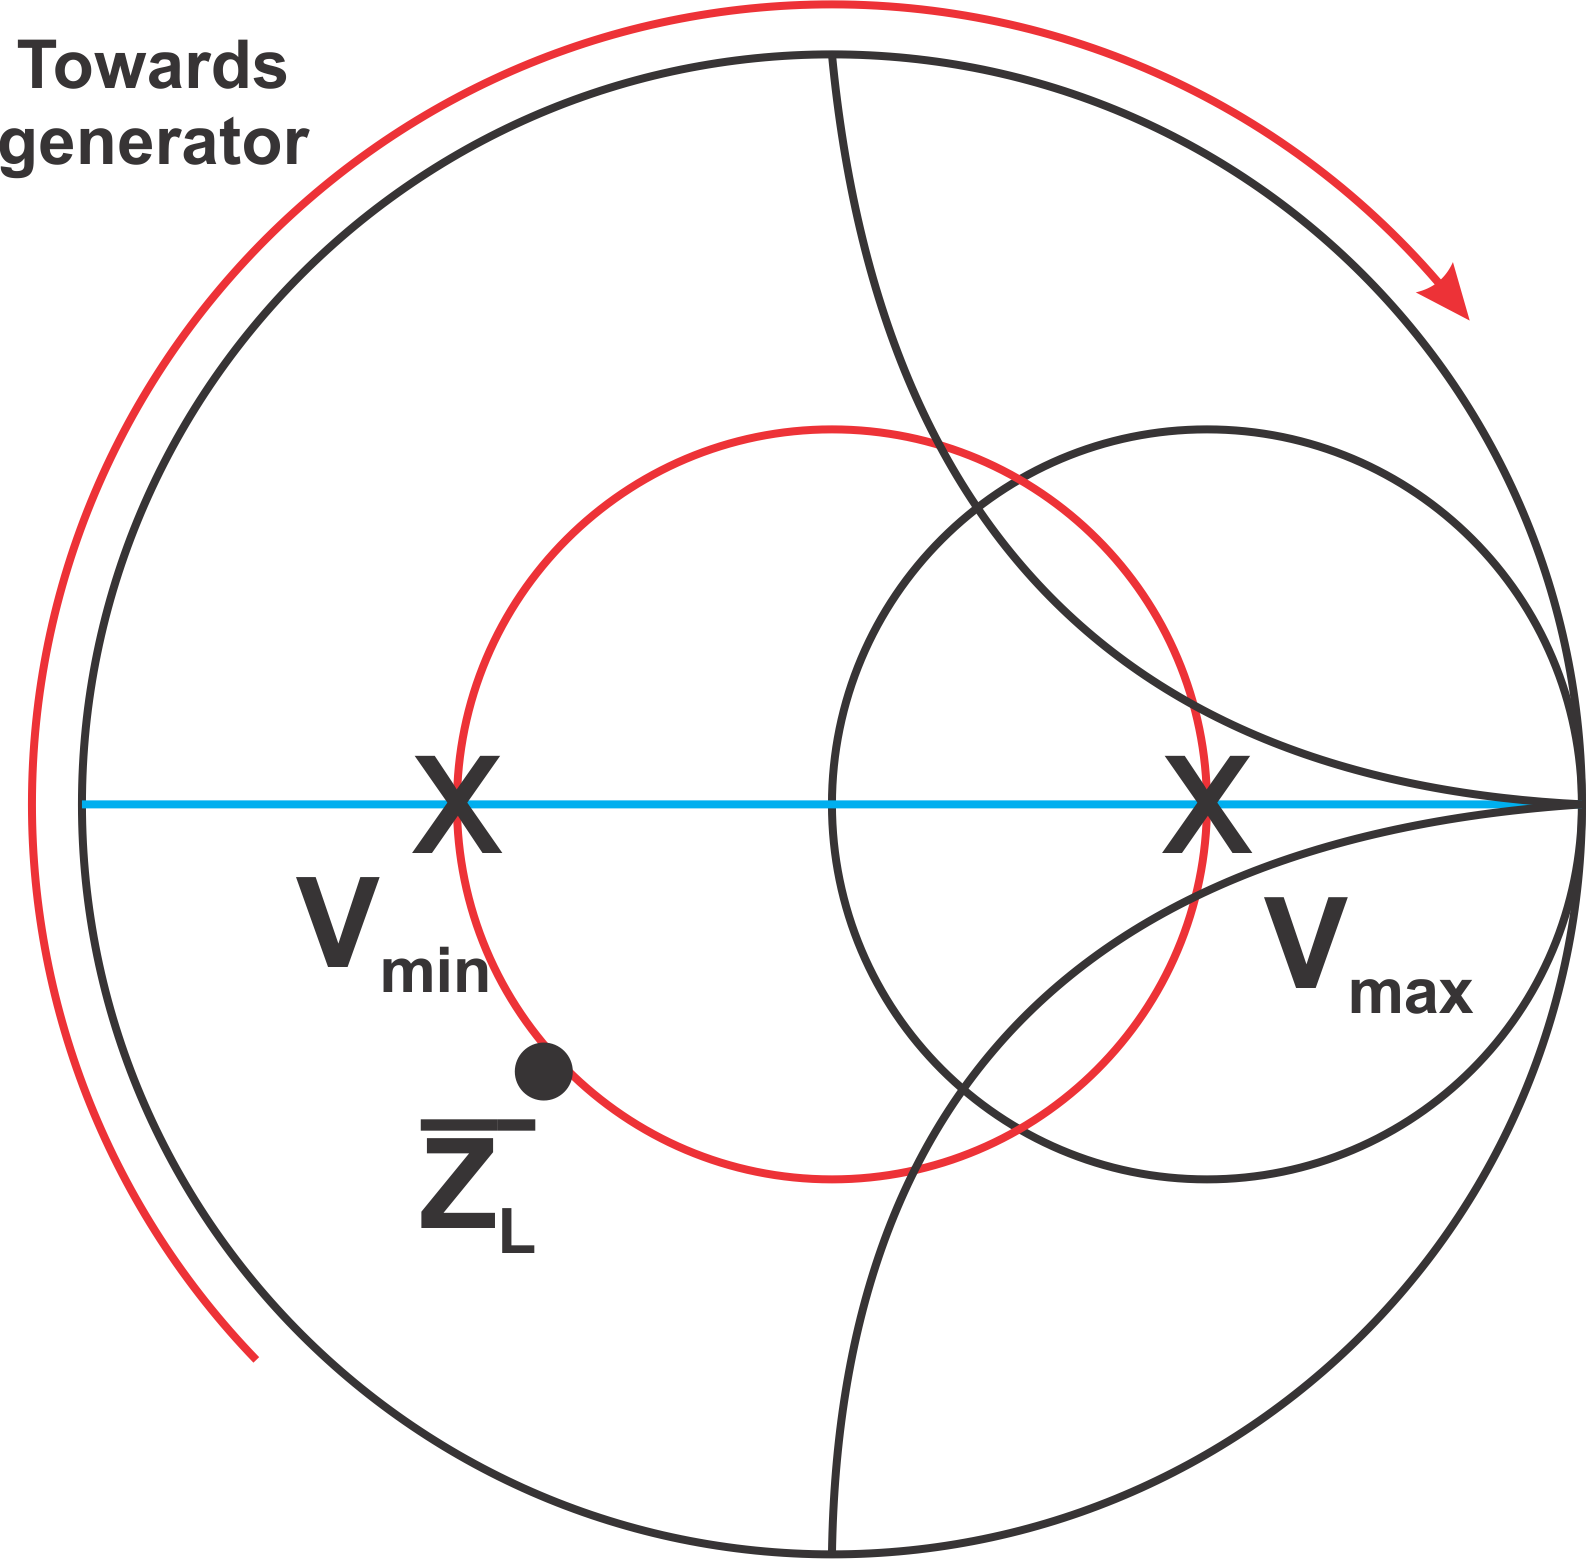
\includegraphics[scale=0.4]{./graphics/Group92}
\caption{A Smith Chart representation of capacitive load}
\label{fig:group92}
\end{figure}

As shown in figure~\ref{fig:group91}, if we move from the load towards the generator, that is, a clockwise rotation, for the inductive load we encounter $V_\max$ first before ${V_\min}$ in another $\frac{\lambda}{4}$ or $\pi rad$ movement. Similarly, if we move from $\bar{Z_L}$ in clockwise direction for capacitive load, we encounter $V_\min$ first before $V_\max$, in another $\frac{\lambda}{4}$ or $\pi rad$ movement. Also, $V_\min\neq0$ which means that for a complex inductive load that is not purely reactive, $VSWR\neq\infty$.

\section{Complex Reactive Loads}
Now, let us analyze some standing wave graph and determine the type of load which they represent. The transmission line circuit is shown in figure~\ref{fig:group93} and we can analyse the standing wave pattern based on the new observation we have discussed. As the standing wave pattern moves from load towards the generator from right to left, it gets to a maximum first and its minimum is not zero so it $|V_\min|$ does not touch the real axis.
\begin{figure}[h]
\centering
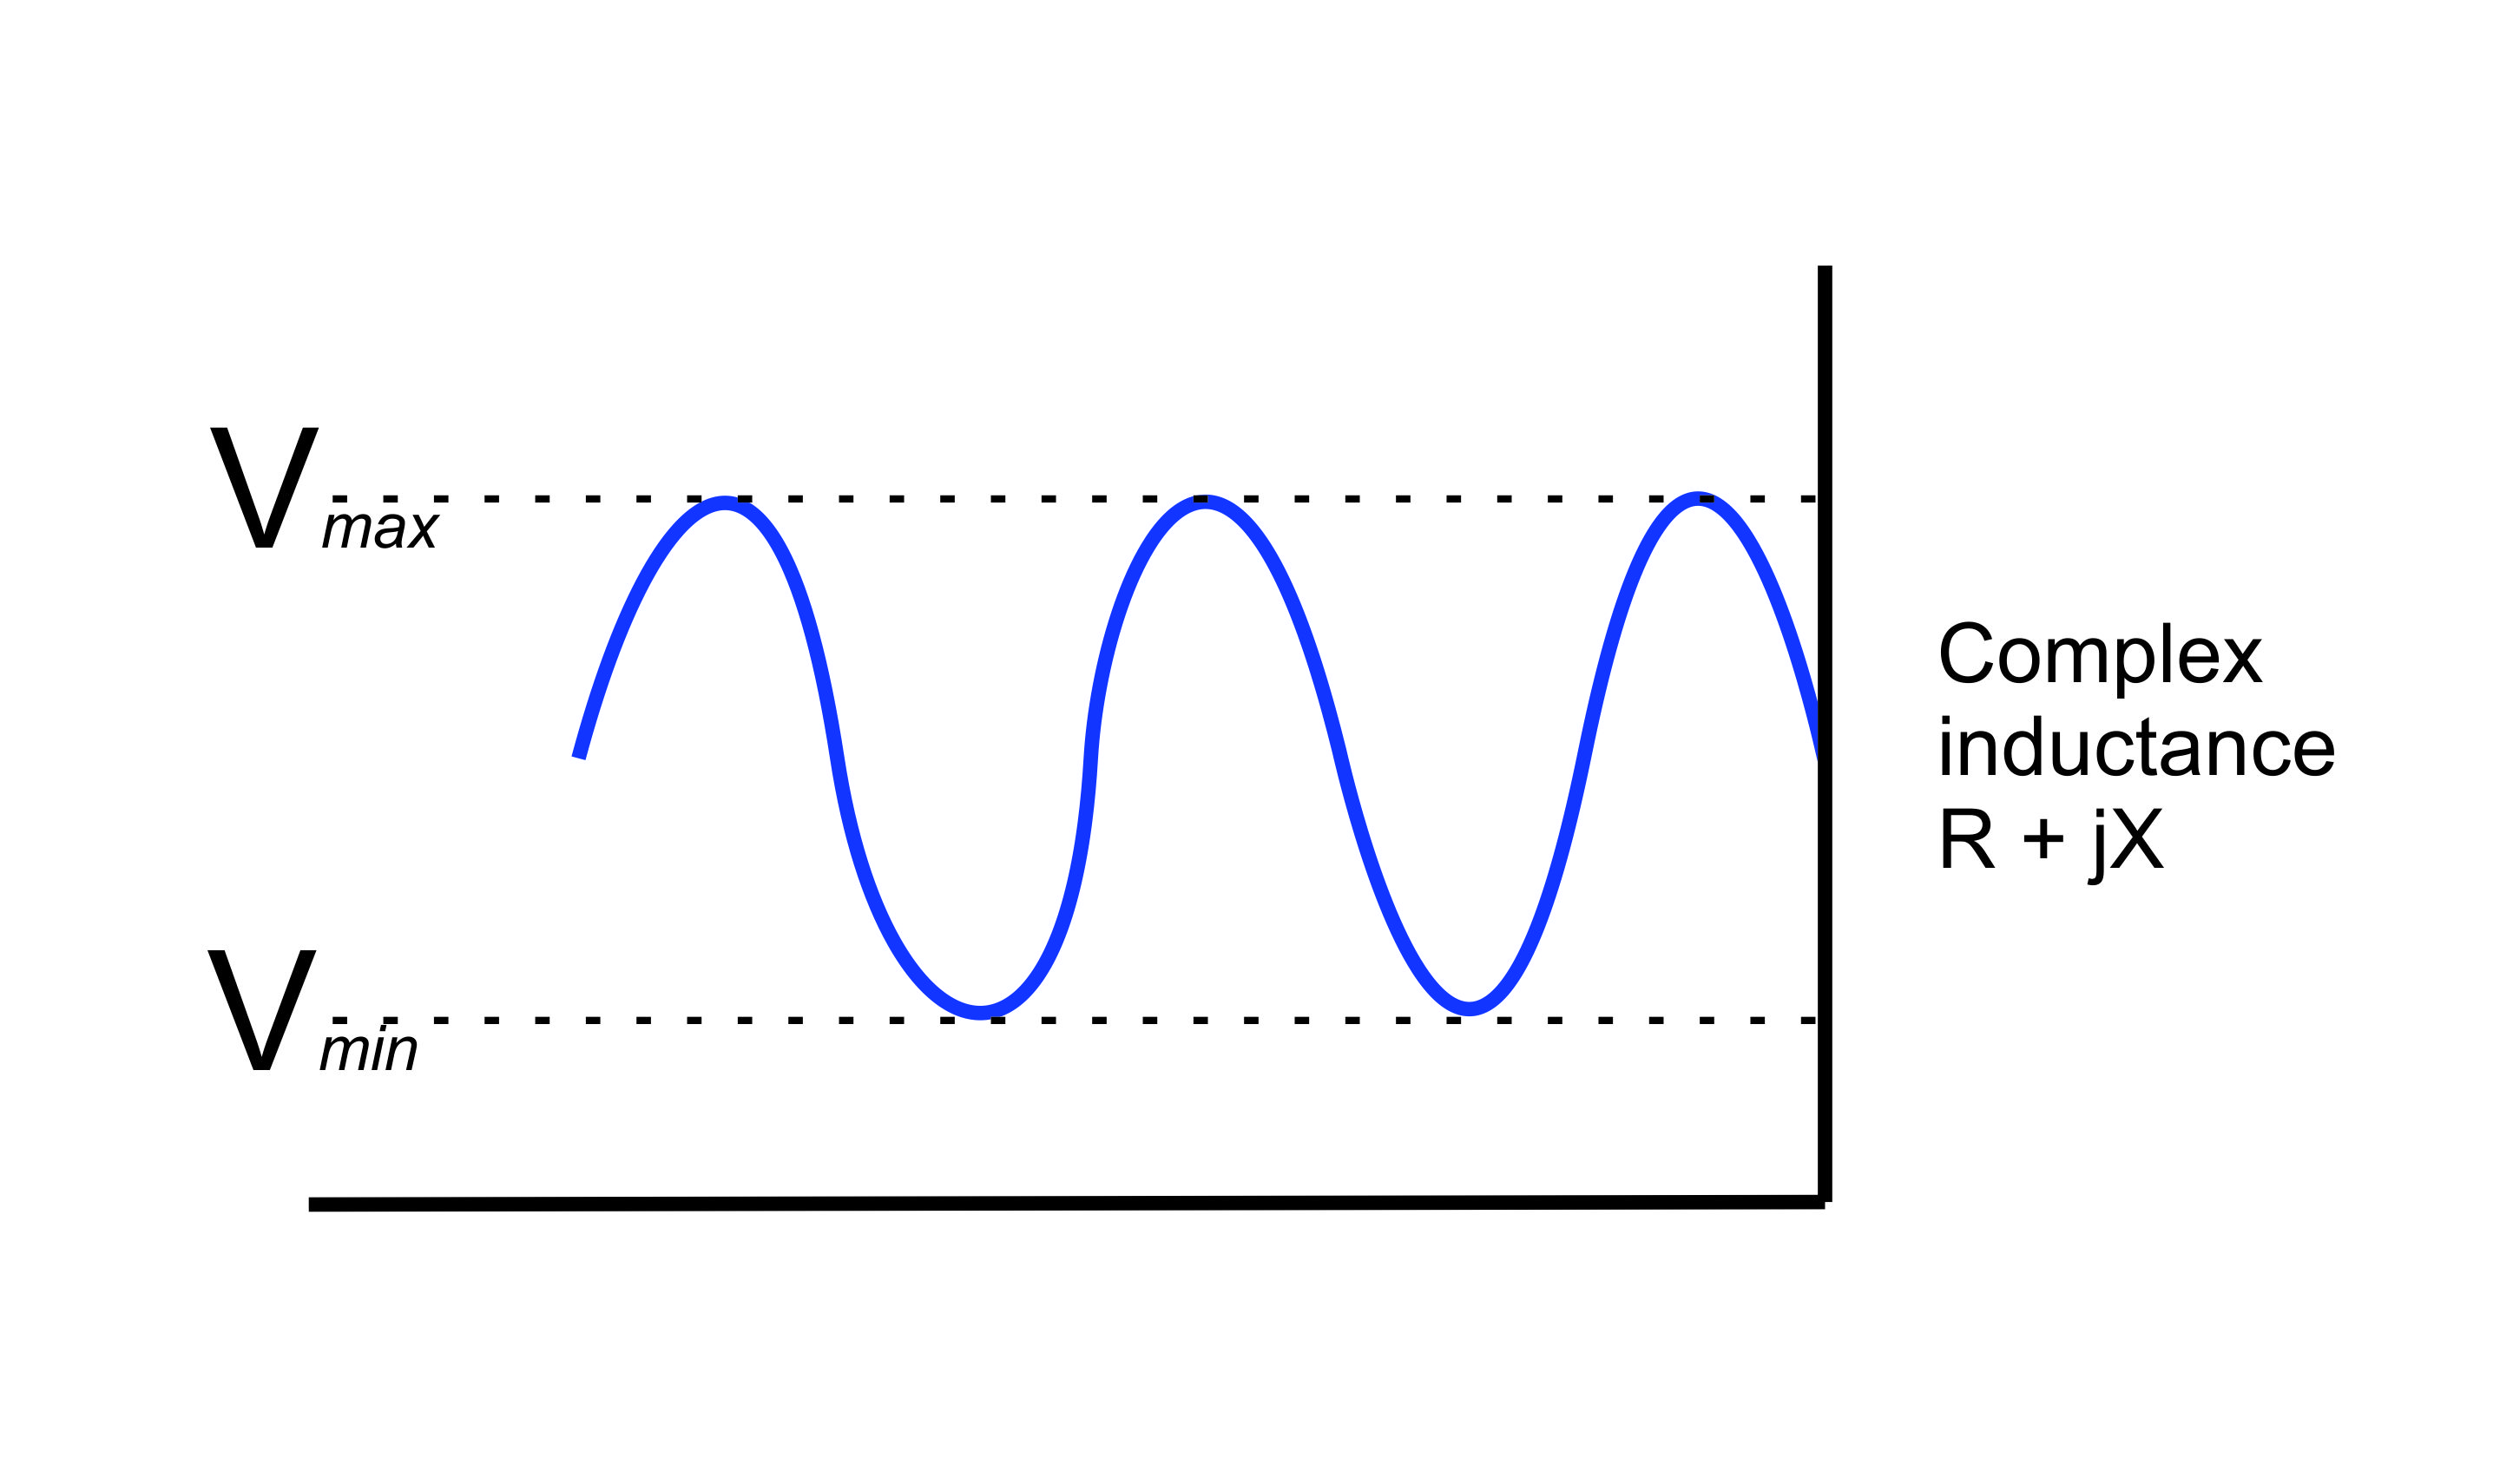
\includegraphics[scale=0.5]{./graphics/Group93}
\caption{Standing wave pattern variation of a complex inductive load}
\label{fig:group93}
\end{figure}
\begin{figure}[h]
\centering
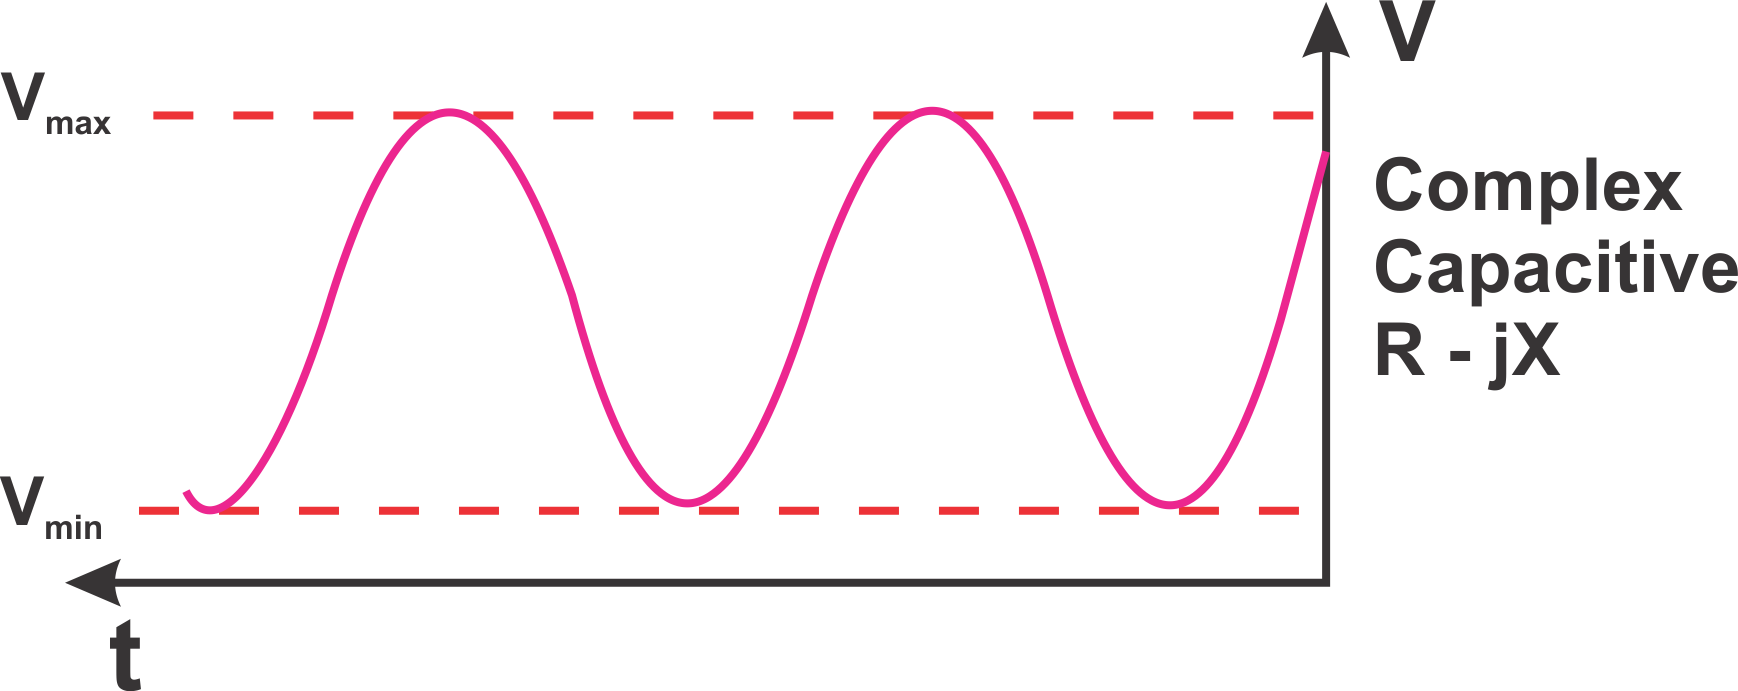
\includegraphics[scale=0.5]{./graphics/Group94}
\caption{Standing wave pattern variation of a complex capacitive load}
\label{fig:group94}
\end{figure}

Similarly for a complex capacitive load, $V_\min\neq0$ and we encounter $V_\min$ first before $V_\max$ as shown in figure~\ref{fig:group94}. 

\section{Purely Reactive Loads}
Let us observe the standing wave patterns with pure reative components at the load end. As shown in figure~\ref{fig:group96}, the voltage minimum is zero or it touches the horizontal axis that is ${VSWR=\dfrac{V_\max}{V_\min}=\infty}$ as ${V_\min=0}$.
\begin{figure}[h]
\centering
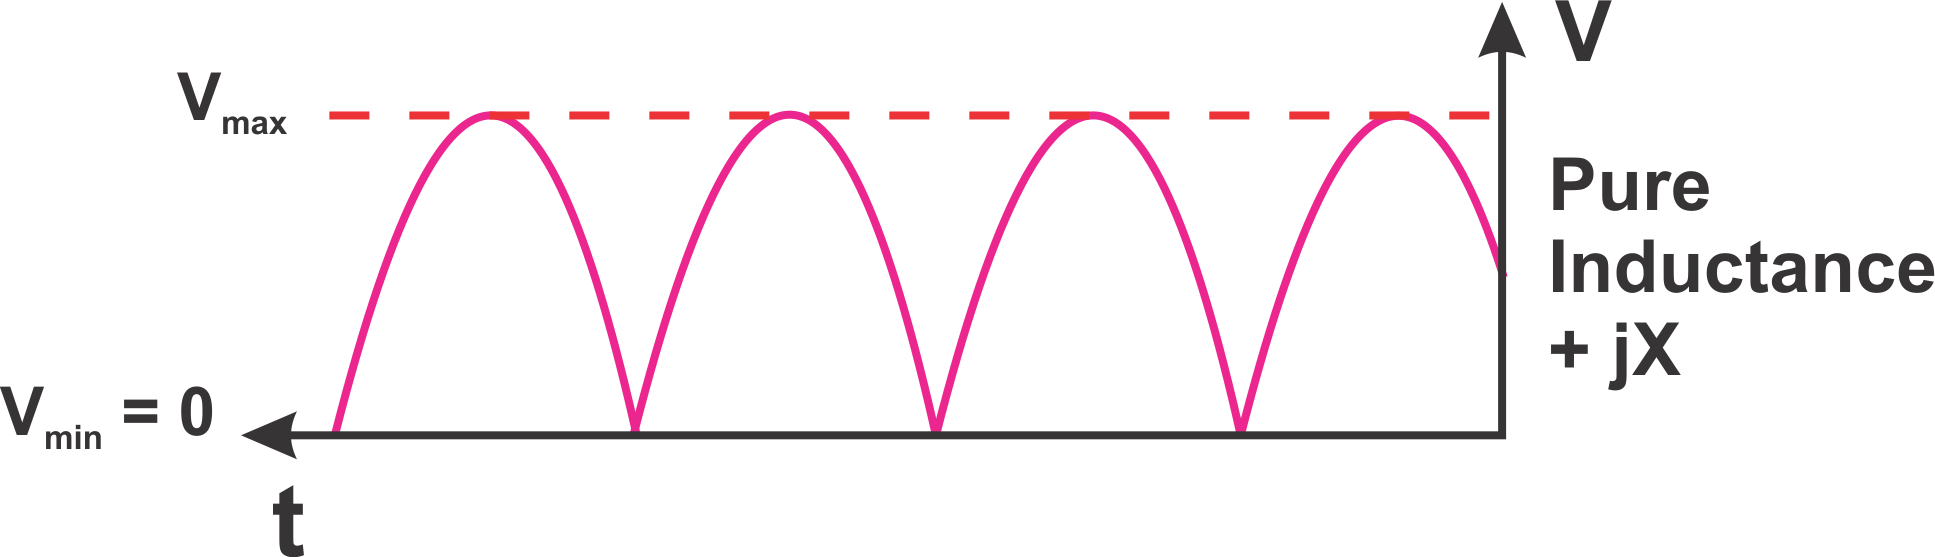
\includegraphics[scale=0.5]{./graphics/Group96}
\caption{Standing wave pattern variation of a pure inductive load}
\label{fig:group96}
\end{figure}

As we move from the load end we meet ${V_\max}$ first indicating it is purely inductive and lies on the upper half of the Smith Chart.
\begin{figure}[h]
\centering
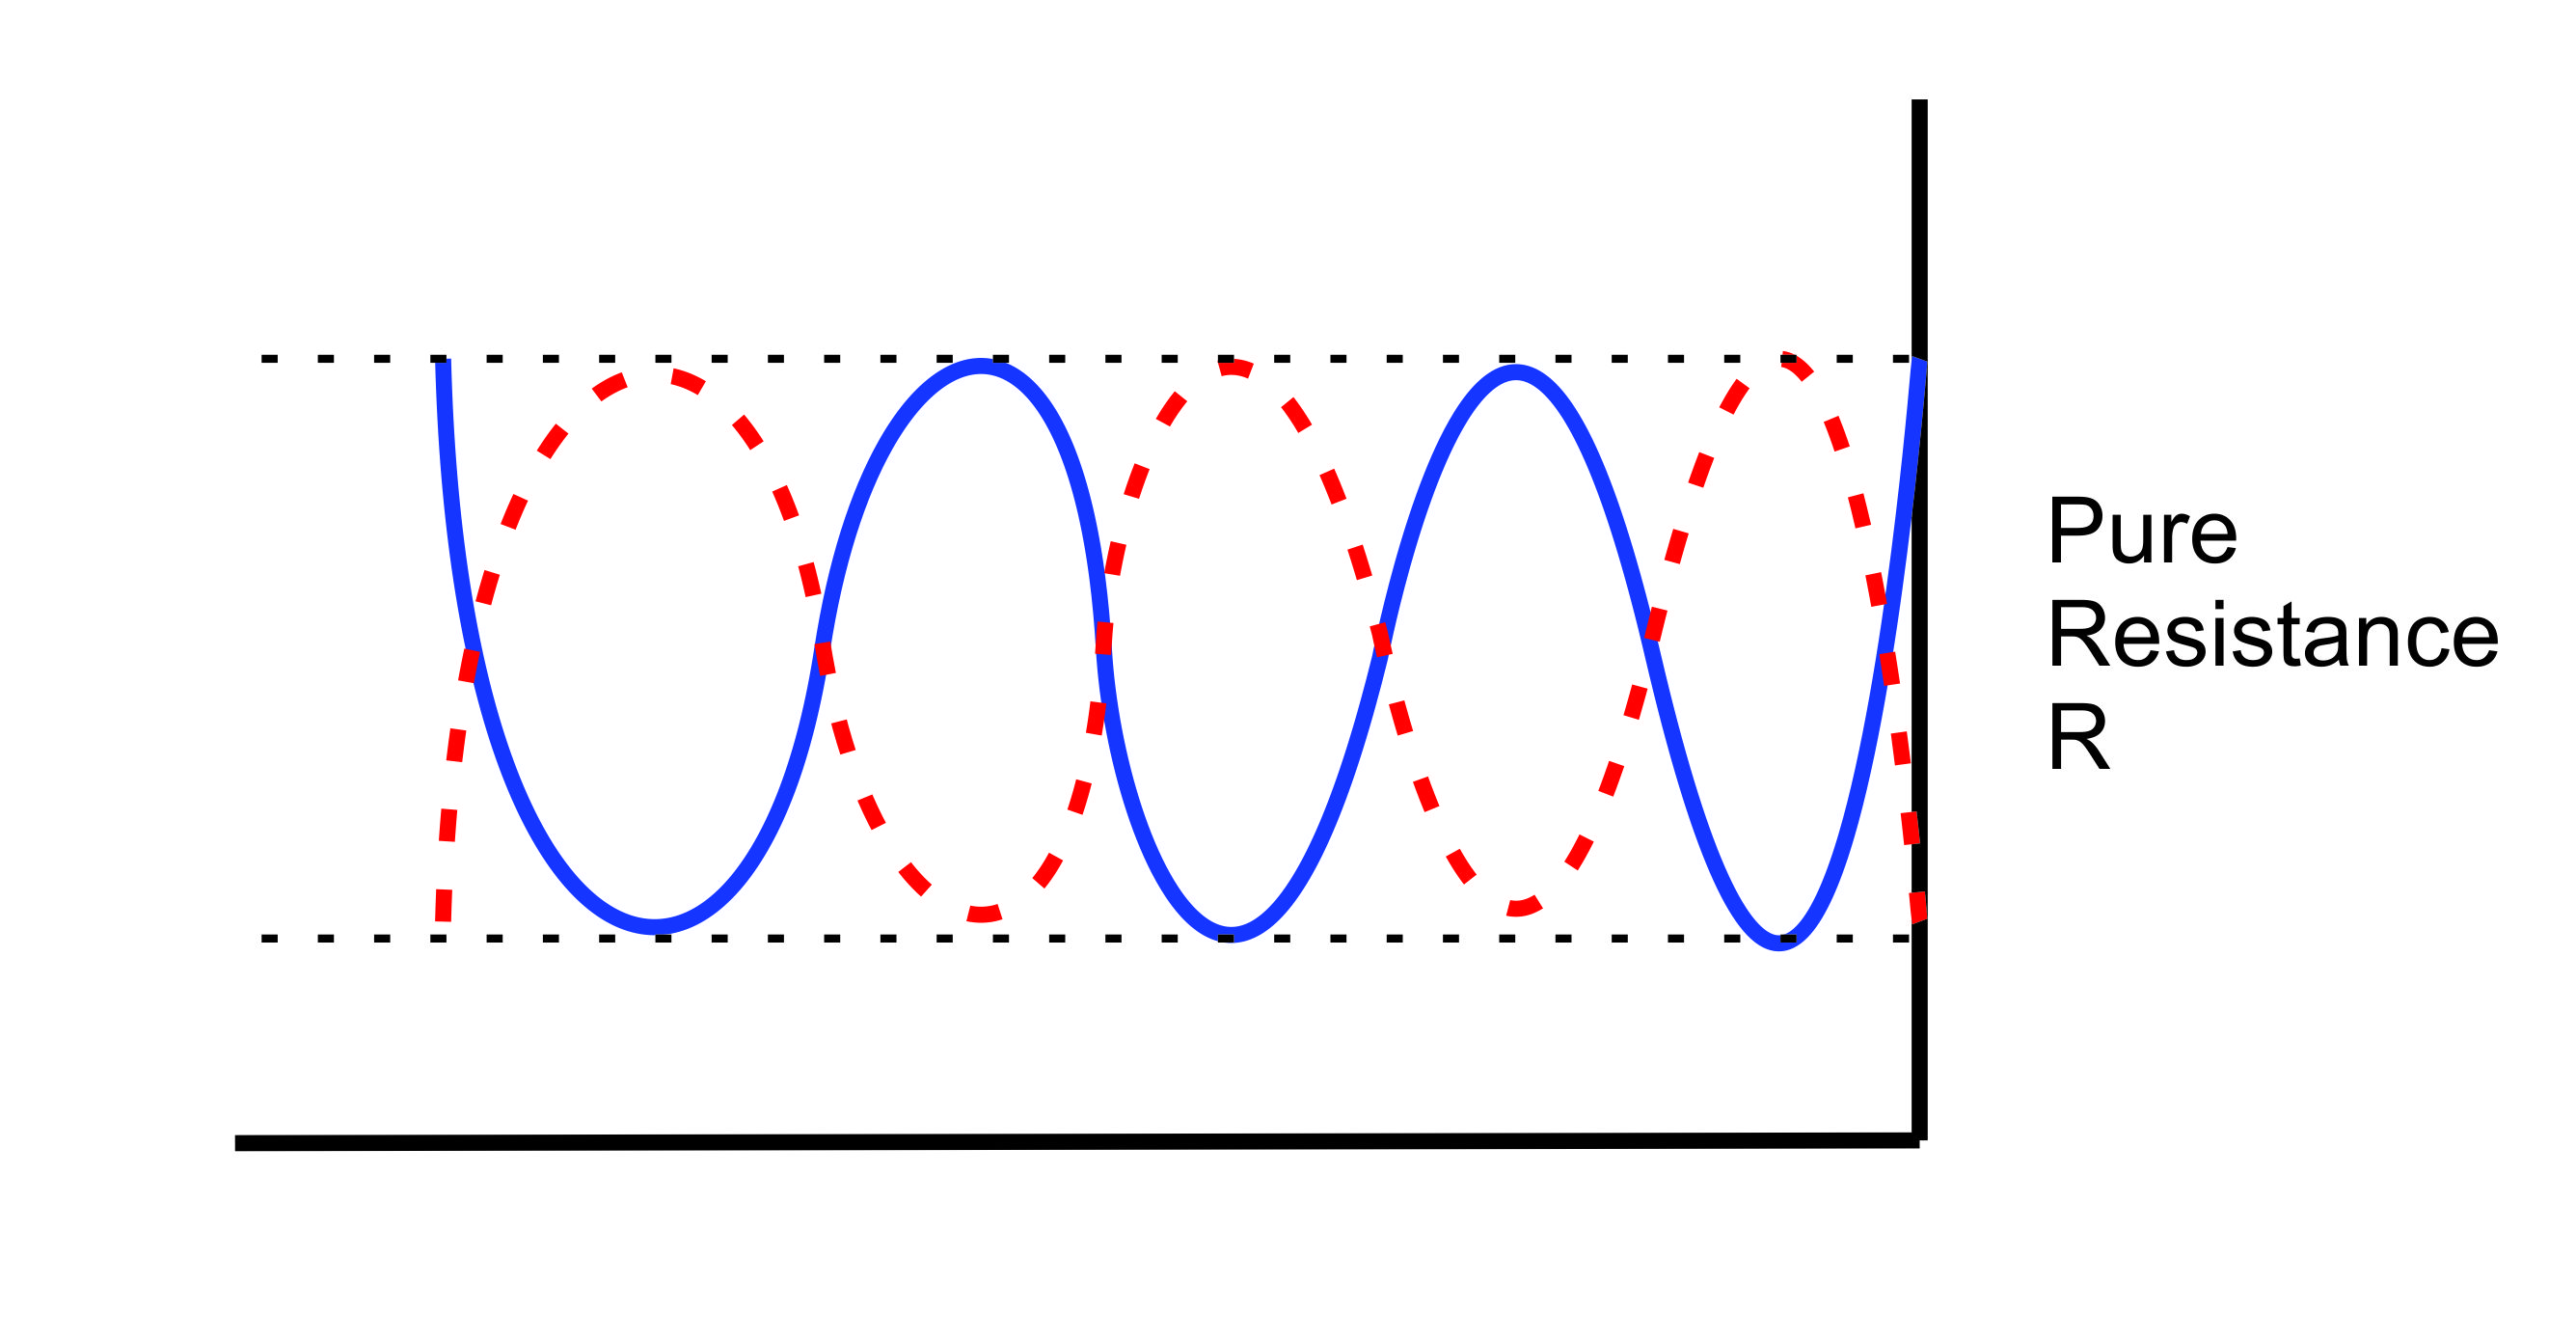
\includegraphics[scale=0.5]{./graphics/Group97}
\caption{Standing wave pattern variation of a pure capacitive load}
\label{fig:group97}
\end{figure}

For purely capacitive loads, the voltage minimum is also zero, but we encounter a minimum first as we go from the load end towards the generator indicating a purely capacitive load. So it lies in the lower half of the Smith Chart and $VSWR=\infty$.

\section{Resistive Loads}
Lastly, there is the case of when the load is neither capacitive nor inductive. If so, then the load must lie on the real horizontal axis of the Smith Chart, so the location of the load itself will be at either the voltage minimum point or voltage maximum point. If the load is purely resistive as in figure~\ref{fig:group95}. Recall that on the Smith Chart, the points of intersection of the VSWR circle on the real axis will be the locations of the voltage maximum and minimum. So there will either be maximum or minimum voltage at the load end as shown in figure~\ref{fig:group95}. The solid curve has ${V_\max}$ at load end meaning ${R>Z_o}$ while the dashed curve has ${V_\min}$ at load end which means ${R<Z_o}$. ${Z_o}$ is the characteristics impedance.
\begin{figure}[h]
\centering
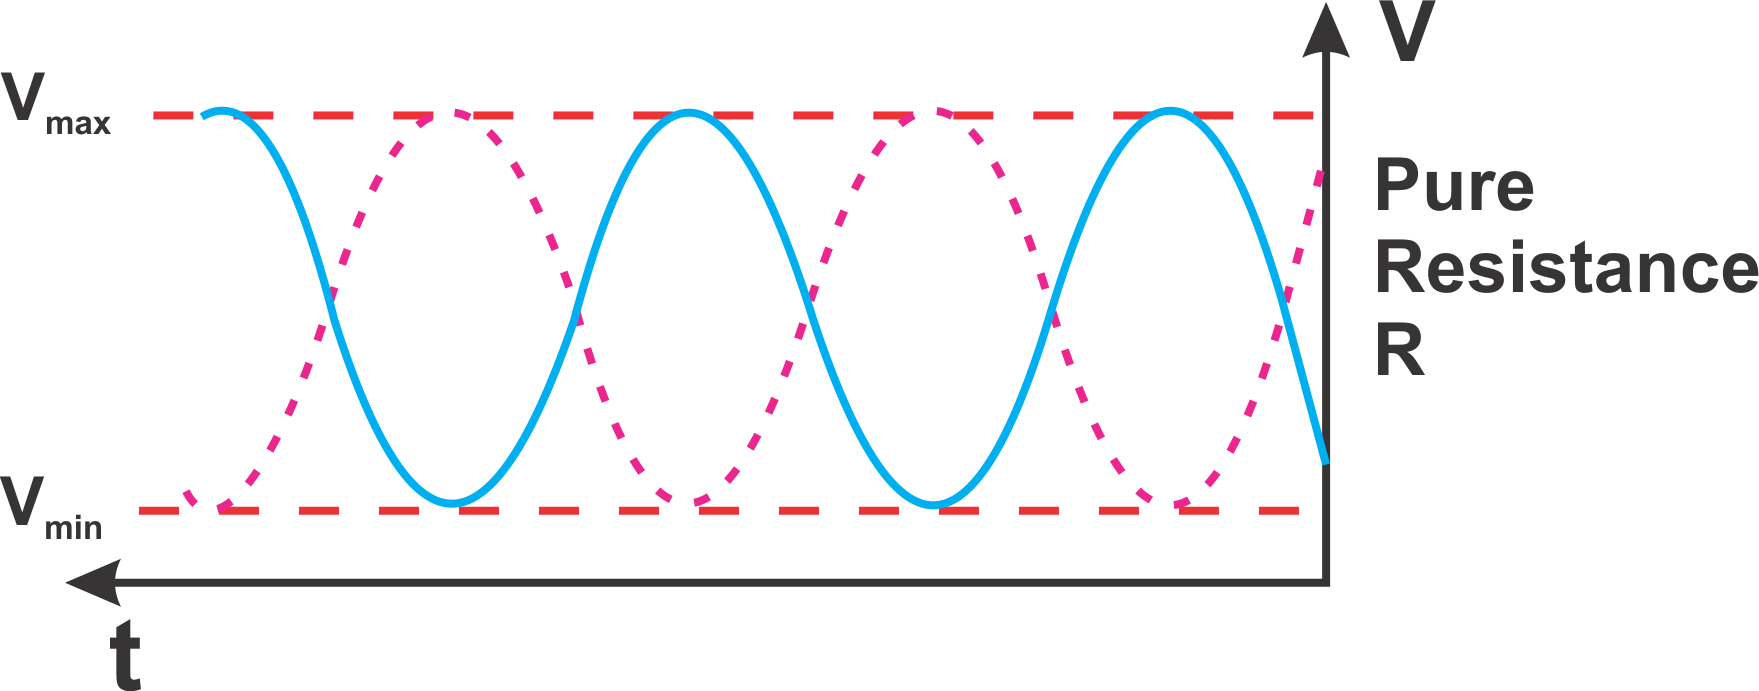
\includegraphics[scale=0.5]{./graphics/Group95}
\caption{Standing wave pattern variation of a pure resistive}
\label{fig:group95}
\end{figure}

So looking at the standing wave pattern, one can quickly identify the types of load because the information about the load is completely available from the standing wave pattern. Hence, ${V_\max}$ and ${V_\min}$ location and lowest value of ${V_\min}$ which is related to VSWR can help us identity loads very quickly.

\section{Transmission line problems}
Now we solve some simple problems based on the theory we have developed from the transmission line.

\section*{Exercises}
\begin{ExerciseList}
\Exercise[label={ex91}]
Explain the following:
\end{ExerciseList}